\documentclass[11pt]{scrartcl}
\usepackage{graphicx}
\graphicspath{{./}}
\usepackage[sexy]{evan}
\usepackage[normalem]{ulem}
\usepackage{hyperref}
\usepackage{mathtools}
\hypersetup{
    colorlinks=true,
    linkcolor=blue,
    filecolor=magenta,      
    urlcolor=cyan,
    pdfpagemode=FullScreen,
    }
\usepackage[most]{tcolorbox}
\renewcommand{\dangle}{\measuredangle}

\renewcommand{\baselinestretch}{1.5}

\addtolength{\oddsidemargin}{-0.4in}
\addtolength{\evensidemargin}{-0.4in}
\addtolength{\textwidth}{0.8in}
% \addtolength{\topmargin}{-0.2in}
% \addtolength{\textheight}{1in} 


\setlength{\parindent}{0pt}

\usepackage{pgfplots}
\pgfplotsset{compat=1.15}
\usepackage{mathrsfs}
\usetikzlibrary{arrows}

\title{Math Without Borders - Grade 2}
\author{Compiled by Azzam (Instagram: @haxuv.world)}
\date{\today}

\begin{document}
\maketitle

\section*{Fast Precise Questions}
\begin{enumerate}
\item What number should we replace $\square$ with, so that
    \[ 41 + 39 = 95 - \square ? \]

\item By how much is the sum of $31+1000$ greater than the difference of
    $31 - 1000$?

\item What digit should we replace $\square$ with, so that
    \[ 7 \text{ tens} + 8 \text{ tens} + 50 \text{ ones} = \square \text{ hundreds}? \]

\item Find the missing number.
    \[ 1, 1, 2, 3, 5, 8, \dots \]

\item How many two-digit numbers are smaller than 90?

\item Which whole even numbers are smaller than 2025 and greater than 2022?

\item Initially, George had 20 books. Nine of them were red, and the rest were yellow. He gave 7 yellow books to his mother. Then he gave 3 yellow books to his friend Maria. How many yellow books does he have left?

\item Harry planted 24 trees in a row. Each 2 trees were planted 1 meter apart. What is the length (in meters) of the row of trees that Harry planted?

\item A triangle has side lengths of 7 cm, 7 cm and 6 cm. A square has a side length of 1 dm. By how many centimetres is the perimeter of the square greater than the perimeter of the triangle?

\item I have two sticks – one with a length of 15 cm and one with a length of 5 cm. I used them to measure the length of a board. I used the stick with a length of 15 cm three times, and I used the stick with a length of 5 cm once. Find the length of the board in cm.

\item Calculate
    \[ (207 + 209 + 211 + 213 + 215 + 217) - (217 + 215 + 213 + 209 + 207) \]

\item The third day of December 2021 falls on a Friday. Which day of the week will the 16\textsuperscript{th} day of December fall on?

\item If
\begin{align*}
    a+b &= 2\\
    b+c &= 3\\
    c+d &= 4\\
    d+a &= 3
\end{align*}
calculate $a+b+c+d$.

\item Calculate $(2015 - 2005 - 2004 - 2003 - 2002 - 2001) + (2001 + 2002 + 2003 + 2004 + 2005)$.

\item In following figure, all the angles given in the following figure are straight angles. Find the area of the figure.
    \begin{figure}[h]
        \centering
        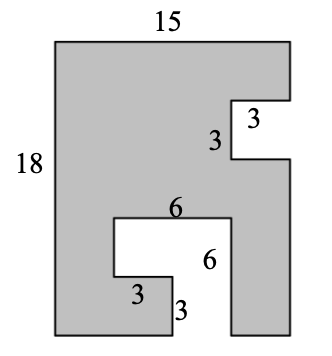
\includegraphics[width=0.4\textwidth]{StarGen/0Figure/nazi-area.png}
    \end{figure}

\item One of the sides of a rectangle has a length of 15 mm, and the other side is 20 mm longer. Find the perimeter of the rectangle in dm.

\item There are 3 points on a straight line. Adam measured the distances between each two of the points and recorded two of them: 1 cm and 5 cm. Find the length of the third distance. Write down all possible answers.

\item How many points should we place on a straight line in order to get exactly 6 line segments?

\item We can use three different weights of 1 kg, 2 kg and $x$ kg in order to weigh each of ten packages weighing between 1 kg and 10 kg on a pair of scales. Find the number $x$.

\item Ivo and Ellie wrote down eleven numbers each. Ivo wrote down 2, 5, 8, ..., 29, 32. Ellie wrote down 11, 14, 17, ..., 38, 41.
    How many of the numbers written down by Ivo were also written down by Ellie?

\item Several children have a total of 20 candies. Five of the children have three candies each, and each of the remaining children has one balloon. How many children are there?

\item What is the greatest difference of two two-digit numbers made up of 4 different digits?

\item Find $\square$, if
    \[ 7+7+7+2 = 4 \times (4 + \square) \]

\item How many two-digit prime numbers with repeated digits are there?

    \item  12 bottles of milk contain 4 litres of milk. How many litres of milk do 45 bottles of milk contain?

    \item  Fritzy had some dumpling. After she ate 2 less than a half of the dumpling, 42 dumpling were left. How many dumpling did Fritzy have at the beginning?

    \item  There are 3 red, 4 yellow, 5 blue and 6 green marbles in a bag. At least how many marbles have to be picked up to ensure that 3 marbles of different colours are picked up?

    
    \item  The sides of each small grey square are 3 centimetres long in the following figure. How many centimetres is the perimeter of the shaded area?
    \begin{figure}[h]
        \centering
        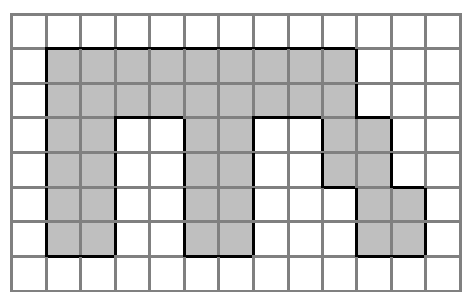
\includegraphics[width=0.4\textwidth]{StarGen/0Figure/perimeter-weird.png}
    \end{figure}
\end{enumerate}



\section*{MATHEMATICAL RELAY}
The answer for each problem is represented by the symbols @, \#, \&, § and *, and must be used to solve each following problem. Each team must fill one answer sheet.

\begin{enumerate}[resume]
\item 4 different digits have been used to write down two odd two-digit numbers with a difference of 2. The greatest possible sum of the two numbers is @. Find @.

\item It takes the ant @ seconds to travel a third of the way. It can travel the whole way in \# minutes. Find \#.

\item The product of five numbers is \#, and their sum is the odd number \&. Find \&.

\item The side of the square ABCD is \& cm. The rectangle AMTD has a side AM, which is a third of the side AD. The square ABCD has a perimeter, which is greater than the perimeter of the rectangle MBCT by § cm. Find §.
\begin{figure}[h]
    \centering
    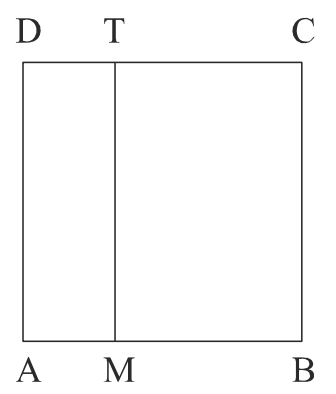
\includegraphics[scale=0.5]{StarGen/0Figure/square-mwb.png}
\end{figure}

\item I chose 4 numbers from 1 to §, such that the product of two of the chosen numbers would be equal to the product of the other two chosen numbers. The sum of the numbers that have not been chosen is *. Find all possible values of *.
\end{enumerate}

\end{document}